\documentclass[conference]{IEEEtran}
\usepackage{amsmath,amssymb,booktabs,graphicx,multirow,url}
\usepackage{algorithm}
\usepackage{algpseudocode}
\usepackage[hidelinks]{hyperref}
\graphicspath{{../results/openmeteo/}{./}}

\begin{document}

\title{Anchor and Median: Why Machine-Learning Models\\Struggle to Beat Persistence for Next-Day PM$_{2.5}$\\in Indian Cities}

% TODO(author): check name/affiliation/e-mail before submission
\author{\IEEEauthorblockN{Kopal Garg}
\IEEEauthorblockA{Indira Gandhi Delhi Technical University for Women, New Delhi, India}}

\maketitle

\begin{abstract}
Machine-learning (ML) forecasts of next-day air quality are usually compared with
other ML models, and less often with the trivial \emph{persistence} forecast
(``tomorrow equals today''). We benchmark eleven forecasters for next-day
daily-mean PM$_{2.5}$ in ten Indian cities over almost three years of
rolling-origin out-of-sample tests (10{,}320 city-days, 2024--2026). Gradient-boosted trees
trained in the standard way (regressing the next-day level under squared loss) are
\emph{worse} than persistence overall (MAE skill $-1.2\%$) and beat it in only
4 of 10 cities. A $2\times2$ factorial ablation shows that two small design
choices interact: (i)~predicting the \emph{change} from persistence and (ii)~training under
\emph{median} (pinball) loss. Each gives little benefit alone ($+0.8\%$ and
$+1.5\%$), but together they give $+6.0\%$, and $+14.9\%$ when next-day
meteorology is available. The resulting model, Persistence-Anchored Quantile
boosting (PAQ), beats persistence in every city and every season, significantly outperforms
standard boosting (Diebold--Mariano $p<10^{-3}$), and, with normalised
split-conformal calibration, gives 90\% prediction intervals with 91.0\% empirical coverage.
Diagnostics show that the gain does not come from predicting the direction of change better.
It comes from implicit shrinkage: the anchored median model makes 32\% smaller moves and loses far less on
calm days. A learned confidence gate that shrinks toward persistence explicitly
adds nothing and is unstable, which we report as a negative result.
\end{abstract}

\begin{IEEEkeywords}
air quality forecasting, PM2.5, persistence baseline, gradient boosting, quantile regression, conformal prediction, India
\end{IEEEkeywords}

%=====================================================================
\section{Introduction}
%=====================================================================
Fine particulate matter (PM$_{2.5}$) is one of the most serious environmental health
problems in Indian cities. In the Indo-Gangetic Plain (IGP), winter concentrations regularly
exceed the national 24-hour standard of 60\,$\mu$g\,m$^{-3}$ by a large margin. The causes
include local emissions, regional transport and episodic agricultural burning
\cite{cusworth2018}. Short-range forecasts, typically one to three days ahead, are the basis for
public health advisories and for triggering emergency emission controls.
Operational forecasts in India come from chemical-transport models such as the
SAFAR system and a high-resolution WRF-Chem system for Delhi \cite{jena2021}.
Global products such as the Copernicus Atmosphere Monitoring Service (CAMS) cover
every Indian city \cite{inness2019}.

In parallel, a large literature applies data-driven methods to the same task,
ranging from support vector machines and neural networks
\cite{masood2020} to tree ensembles \cite{natarajan2024,maltare2023} and deep
sequence models \cite{pruthi2022,huang2018,zhou2024}. These models are almost always
evaluated against each other, with $R^2$, RMSE or classification accuracy, and often on
random train/test splits. A recent systematic mapping of 409 air-quality forecasting
studies stresses that reported skill depends heavily on validation design and
horizon, not only on architecture \cite{chianese2026}.

The \emph{persistence} forecast, $\hat y_{t+1}=y_t$, is the standard reference in
weather forecasting \cite{murphy1988,rasp2020} and in forecasting research more
broadly \cite{hyndman2006}. It is especially hard to beat at short horizons for
strongly autocorrelated quantities. Daily log-PM$_{2.5}$ in our ten cities has
lag-1 autocorrelation between 0.82 and 0.95. A model can therefore reach a high $R^2$ simply
because yesterday's value is a good predictor, while still being \emph{less} accurate
than repeating it. If a forecast does not beat persistence, it adds no value to an advisory system.

This paper asks a deliberately simple question: \emph{does a typical ML pipeline
beat persistence for next-day PM$_{2.5}$ in Indian cities and, if not, what is the
smallest change that makes it do so?} Our contributions are:
\begin{enumerate}
\item A reproducible ten-city, rolling-origin benchmark of eleven forecasters
against persistence and climatology, with Diebold--Mariano significance tests, in
two information settings (with and without next-day meteorology).
\item A $2\times2$ factorial ablation (target: level vs.\ change; loss: squared vs.\
median) showing a super-additive \emph{interaction}: together the two ingredients gain
more than the sum of their individual gains.
\item PAQ, a persistence-anchored multi-quantile booster with normalised
split-conformal intervals. It beats persistence in all ten cities, all four seasons and
all three test years.
\item A mechanism analysis that explains \emph{why} the combination works, and a
documented negative result: an explicit learned shrinkage gate is redundant with, and less
stable than, the implicit shrinkage of the median loss.
\end{enumerate}
The rest of the paper is organised as follows. Section~\ref{sec:rw} reviews related
work, Section~\ref{sec:data} describes the data, Section~\ref{sec:method} presents
the forecasters and PAQ, and Section~\ref{sec:setup} the evaluation protocol.
Section~\ref{sec:results} reports the results, and Section~\ref{sec:disc} discusses
implications and limitations.

%=====================================================================
\section{Literature Review}\label{sec:rw}
%=====================================================================
\subsection{Process-based air-quality forecasting in India}
Chemical-transport models (CTMs) simulate emission, transport, chemistry and
deposition explicitly. Over Delhi, a WRF-Chem system with 400\,m innermost grid spacing
produces 72-hour forecasts and detects more than 90\% of unhealthy-air events
\cite{jena2021}. Globally, CAMS assimilates satellite observations of aerosol and trace gases into
the ECMWF forecasting system \cite{inness2019}. Agricultural fires in north-west India
are a major, episodic contributor to Delhi's post-monsoon pollution \cite{cusworth2018}.
This makes episode onset hard to forecast from local history alone. CTMs are physically
grounded but computationally expensive and sensitive to emission inventories. This
motivates statistical post-processing and data-driven alternatives.

\subsection{Machine learning for PM$_{2.5}$ and AQI in India}
Masood and Ahmad \cite{masood2020} compared support vector machines and artificial
neural networks for daily PM$_{2.5}$ in Delhi using meteorological and pollutant
inputs from 2016--18, and found that the ANN was more accurate. Agarwal and Sahu
\cite{agarwal2023} applied statistical time-series models to PM$_{2.5}$ in
Bengaluru and Delhi. Pruthi and Liu \cite{pruthi2022} proposed a low-cost,
nature-inspired deep-learning system for PM$_{2.5}$ forecasting over Delhi. For the
composite AQI, Maltare and Vahora \cite{maltare2023} compared ML models for
Ahmedabad. Natarajan et al.\ \cite{natarajan2024} combined grey-wolf optimisation with a
decision tree on the public Kaggle/CPCB city-day data for six major cities, and reported
$R^2$, RMSE, MAE and accuracy against k-nearest-neighbour, random-forest and
support-vector baselines. Studies in this line usually compare one ML model with other ML
models. Our work instead fixes the comparison to persistence, the baseline an operational
forecaster would actually replace.

\subsection{Deep and spatio-temporal models}
Outside India, research has moved towards deep architectures. Huang and Kuo
\cite{huang2018} combined CNN and LSTM layers for PM$_{2.5}$ forecasting in smart
cities. PM2.5-GNN \cite{wang2020gnn} encodes domain knowledge of transport between
cities in a graph neural network. Reviews of ML for outdoor air quality
\cite{rybarczyk2018,bai2018} and of deep-learning architectures for PM$_{2.5}$
\cite{zhou2024} document a strong trend towards LSTM, CNN, hybrid-decomposition and
graph models. Zhou et al.\ note that many such models fall short on interpretability
\cite{zhou2024}. A mapping review of 409 studies concludes that transparent
statistical and tabular baselines should be the default starting point for short or sparse
single-station records \cite{chianese2026}. Our results support this view: a
tree-based model with a carefully chosen target and loss is a strong, interpretable
reference.

\subsection{Baselines, skill scores and evaluation}
Skill scores relative to a reference forecast are standard in meteorology
\cite{murphy1988}. WeatherBench, a benchmark for data-driven weather prediction, reports
persistence and climatology as reference baselines \cite{rasp2020}. In the forecasting
literature, Hyndman and Koehler \cite{hyndman2006} proposed scaling errors by the
in-sample naive (persistence) forecast. Makridakis et al.\ \cite{makridakis2018} showed that
sophisticated ML methods frequently fail to beat simple statistical benchmarks. For
comparing two forecasts, the Diebold--Mariano (DM) test \cite{diebold1995}, with the
small-sample correction of Harvey et al.\ \cite{harvey1997}, is the standard
significance test.

\subsection{Uncertainty quantification}
Quantile regression \cite{koenker1978} estimates conditional quantiles by minimising
the pinball loss and is natively supported by gradient-boosting libraries
\cite{chen2016}. Murad et al.\ \cite{murad2021} compared Bayesian neural networks,
Monte-Carlo dropout and deep ensembles for probabilistic PM forecasting, and found that
well-calibrated uncertainty supports risk-aware decisions. Conformal prediction
\cite{lei2018} gives distribution-free, finite-sample coverage guarantees under
exchangeability. Conformalised quantile regression \cite{romano2019} combines it with
quantile models so that interval width adapts to the input. PAQ uses a normalised
conformal score built from the spread of its own quantile outputs.

\textbf{Research gap.} We are not aware of a multi-city Indian study that (a)~evaluates
next-day PM$_{2.5}$ forecasters against persistence with significance tests under a
strictly chronological protocol, (b)~isolates \emph{which} design choices make tree
models beat persistence, and (c)~explains the mechanism.

%=====================================================================
\section{Study Area and Data}\label{sec:data}
%=====================================================================
\textbf{Cities.} We study ten cities chosen to span India's pollution and climate
gradients. Four lie in or at the edge of the IGP (Delhi, Lucknow, Patna, Kolkata).
Six are in western, central and southern India (Ahmedabad, Mumbai, Pune, Hyderabad,
Bengaluru, Chennai). The IGP is bounded by the Himalaya, has shallow winter boundary layers
and is affected by crop-residue burning. The southern and coastal cities are ventilated by
sea breezes and the monsoon.

\textbf{Air quality.} Hourly PM$_{2.5}$ comes from the CAMS global
atmospheric-composition forecasting system \cite{inness2019}, retrieved through the
Open-Meteo Air Quality API \cite{openmeteo} for 1~Aug~2022 to 28~Oct~2026 at the grid
point nearest each city centre. Daily means are taken over local (IST) days. Days with
fewer than 18 valid hours are treated as missing.

\textbf{Meteorology.} Hourly ERA5 reanalysis \cite{hersbach2020} provides 2-m
temperature, relative humidity, precipitation, surface pressure, 10-m wind
(converted to $u,v$ components) and boundary-layer height (BLH). These are aggregated to daily
means, plus the daily precipitation sum, BLH minimum and maximum, and diurnal temperature range.
All data are free and require no registration.

\begin{table}[t]
\centering
\caption{Daily PM$_{2.5}$ statistics, Aug 2022 -- Oct 2026 (1{,}547 days per city). $>$60: share of days above the 24-h national standard; $\rho_1$: lag-1 autocorrelation of $\log(\mathrm{PM}_{2.5}+1)$.}
\label{tab:data}
\setlength{\tabcolsep}{4pt}
\begin{tabular}{llrrrrr}
\toprule
City & Region & Mean & SD & P95 & $>$60 (\%) & $\rho_1$ \\
\midrule
Delhi     & IGP   & 74.2 & 37.2 & 148.4 & 56.6 & 0.83 \\
Patna     & IGP   & 61.2 & 37.5 & 137.4 & 40.6 & 0.87 \\
Lucknow   & IGP   & 57.7 & 34.0 & 128.4 & 35.4 & 0.87 \\
Kolkata   & IGP   & 57.6 & 43.1 & 143.6 & 38.3 & 0.91 \\
Mumbai    & Other & 40.1 & 28.9 &  95.8 & 20.9 & 0.91 \\
Ahmedabad & Other & 29.5 & 15.8 &  61.2 &  5.4 & 0.85 \\
Hyderabad & Other & 28.3 & 16.4 &  57.1 &  3.3 & 0.91 \\
Pune      & Other & 27.5 & 18.8 &  60.7 &  5.4 & 0.95 \\
Chennai   & Other & 22.7 & 11.6 &  45.8 &  0.5 & 0.82 \\
Bengaluru & Other & 20.8 & 12.6 &  42.8 &  0.1 & 0.90 \\
\bottomrule
\end{tabular}
\end{table}

Table~\ref{tab:data} summarises the series. Delhi exceeds the national standard on
57\% of days, compared with under 1\% in Bengaluru and Chennai. All series are strongly
persistent ($\rho_1\ge0.82$). This persistence is the reason the naive forecast is a
strong reference.

%=====================================================================
\section{Methods}\label{sec:method}
%=====================================================================
\subsection{Problem formulation}
Let $y_t$ be the daily-mean PM$_{2.5}$ on day $t$ and $z_t=\log(y_t+1)$. A forecast is
issued at the end of day $t$ for day $t+1$. All models predict $z_{t+1}$, and forecasts are
converted back with $\hat y=\exp(\hat z)-1$. The log transform stabilises variance
across cities whose levels differ by a factor of 3.5. Because the exponential is monotone,
a median forecast of $z$ maps to a median forecast of $y$, which is the
MAE-optimal point forecast.

\subsection{Features}
The input vector $x_t$ contains:
(i)~\emph{pollution history}: lags $z_{t-k}$ for $k=0,\dots,6$; one- and two-day differences;
rolling means over 3, 7, 14 and 30 days; the 7-day standard deviation, minimum and maximum; and
anomalies of $z_t$ relative to the 7- and 30-day means.
(ii)~\emph{Day-$t$ meteorology}: all variables from Section~\ref{sec:data}, and the
day-over-day change in BLH, wind speed, temperature, humidity, precipitation and pressure.
(iii)~\emph{Calendar}: sine and cosine of the target day-of-year, and target day-of-week.
In the \emph{perfect-prog} setting we add (iv)~day-$(t{+}1)$ meteorology and its change from
day $t$. Short gaps of at most two days in the pollution history are linearly interpolated for
feature construction only. Targets and the persistence anchor always use the raw series.

\textbf{Settings.} \emph{Nowcast} uses only information available at the end of day
$t$. \emph{Perfect-prog} uses ERA5 for day $t{+}1$ as a stand-in for a skilful
numerical weather forecast. This gives an upper bound on what weather forecasts can add.

\subsection{Baseline forecasters}
\begin{itemize}
\item \textbf{Persistence}: $\hat z_{t+1}=z_t$.
\item \textbf{Climatology}: mean training $z$ within $\pm15$ days of the target
day-of-year.
\item \textbf{Ridge-AR}: ridge regression on all features (median imputation,
standardisation, penalty selected by leave-one-out CV over $10^{-2}$--$10^{3}$).
\item \textbf{RF}: random forest \cite{breiman2001}, 300 trees, minimum leaf size 5,
50\% of features per split.
\item \textbf{XGB-level}: gradient boosting \cite{chen2016} on the level $z_{t+1}$
with squared loss. This is the standard pipeline in the literature.
\item \textbf{Factorial variants}: XGB-level (median), XGB-change and XGB-change
(median). These complete the $2\times2$ design over target and loss.
\end{itemize}
All boosted models share one hyperparameter set (Table~\ref{tab:hp}). Nothing was tuned on the
test years.

\begin{table}[t]
\centering
\caption{Shared gradient-boosting hyperparameters (XGBoost 3.0, \texttt{hist}).}
\label{tab:hp}
\begin{tabular}{lr|lr}
\toprule
Trees & 500 & Subsample & 0.8 \\
Learning rate & 0.03 & Column subsample & 0.8 \\
Max depth & 4 & Min.\ child weight & 5 \\
L2 penalty $\lambda$ & 1.0 & Quantiles (PAQ) & 0.1, 0.5, 0.9 \\
\bottomrule
\end{tabular}
\end{table}

\subsection{PAQ: Persistence-Anchored Quantile boosting}
PAQ fits a single multi-output quantile booster to the \emph{change}
$\Delta_t=z_{t+1}-z_t$ at $\tau\in\{0.1,0.5,0.9\}$ by minimising the pinball loss
\cite{koenker1978}
\begin{equation}
\mathcal L_\tau(\Delta,\hat q)=\max\{\tau(\Delta-\hat q),\,(\tau-1)(\Delta-\hat q)\}.
\end{equation}
The point forecast and the spread are
\begin{equation}
\hat z_{t+1}=z_t+\hat q_{0.5}(x_t),\qquad w(x_t)=\hat q_{0.9}(x_t)-\hat q_{0.1}(x_t).
\end{equation}
Two properties motivate this design. First, persistence is the model's \emph{default}:
an uninformative model ($\hat q_{0.5}\equiv0$) reproduces persistence exactly. A level model,
in contrast, must relearn the identity mapping $z_t\mapsto z_{t+1}$ from data, and a regularised
tree ensemble does this only approximately. Second, the conditional median of a distribution
sharply peaked at zero lies closer to zero than its conditional mean whenever large changes are
asymmetric or heavy-tailed. The median loss therefore leads to more conservative moves away from
persistence (Section~\ref{sec:mech}).

\textbf{Calibrated intervals.} For prediction intervals we use split-conformal
calibration \cite{lei2018,romano2019} with cross-fitting. The training period is split
into $K=4$ contiguous blocks. For each block, a quantile model is trained on the other three and
predicts the held-out block, which gives out-of-fold (OOF) forecasts $\hat z_i$ and spreads $w_i$
for every training day. The normalised conformity score is $r_i=|z_i-\hat z_i|/w_i$. With $\hat c$
the $\lceil(n+1)(1-\alpha)\rceil/n$ empirical quantile of $\{r_i\}_{i=1}^n$, the
$(1-\alpha)$ interval is
\begin{equation}
\left[\exp(\hat z_{t+1}-\hat c\,w(x_t))-1,\ \exp(\hat z_{t+1}+\hat c\,w(x_t))-1\right].
\end{equation}
It is asymmetric in concentration units and widens multiplicatively with the level. We also report
an \emph{absolute} variant with $r_i=|z_i-\hat z_i|$ (constant width in log space). The final
quantile model is refitted on the whole training period. Algorithm~\ref{alg:paq} summarises the
procedure.

\begin{algorithm}[t]
\caption{PAQ training and forecasting}\label{alg:paq}
\begin{algorithmic}[1]
\Require training days $\{(x_i,z_i,z_{i+1})\}_{i=1}^n$ in time order, miscoverage $\alpha$
\State $\Delta_i\gets z_{i+1}-z_i$
\For{$k=1,\dots,K$} \Comment{contiguous blocks $B_k$}
  \State fit quantile booster $Q^{(-k)}$ on $\{(x_i,\Delta_i)\}_{i\notin B_k}$
  \State $(\hat q_{.1},\hat q_{.5},\hat q_{.9})_i\gets\mathrm{sort}(Q^{(-k)}(x_i))$ for $i\in B_k$
\EndFor
\State $r_i\gets|z_{i+1}-z_i-\hat q_{.5,i}|/(\hat q_{.9,i}-\hat q_{.1,i})$
\State $\hat c\gets$ the $\lceil(n+1)(1-\alpha)\rceil$-th smallest $r_i$
\State fit $Q$ on all $\{(x_i,\Delta_i)\}$
\State \textbf{Forecast} for new $x_t$: $(\hat q_{.1},\hat q_{.5},\hat q_{.9})\gets\mathrm{sort}(Q(x_t))$
\State \Return $\hat z_{t+1}=z_t+\hat q_{.5}$, \ interval $\hat z_{t+1}\pm\hat c(\hat q_{.9}-\hat q_{.1})$
\end{algorithmic}
\end{algorithm}

\subsection{Gated variants (ablation)}
If PAQ helps by being conservative, an explicit, learned shrinkage might help further.
We tested
\begin{equation}
\hat z_{t+1}=z_t+\gamma(x_t)\,\hat q_{0.5}(x_t),
\end{equation}
with either a constant gate $\gamma=\sigma(a)$ or a confidence gate
$\gamma=\sigma(a+b\log s)$, where $s=|\hat q_{0.5}|/w$ is the signal-to-noise ratio
(SNR) of the predicted change and $\sigma$ is the logistic function. The hypothesis was
$b>0$: move away from persistence only when the predicted change is large relative to
its uncertainty. The parameters $(a,b)$ are fitted on the OOF predictions by minimising MAE in
concentration units (Nelder--Mead, three restarts).

%=====================================================================
\section{Experimental Setup}\label{sec:setup}
%=====================================================================
\textbf{Protocol.} We use expanding-window rolling-origin evaluation for each city.
Models are trained separately per city. For test year $Y\in\{2024,2025,2026\}$, each model is
trained on all days before 1~January~$Y$ and evaluated on every day of $Y$ (2026 runs to
28~October). Training sets therefore grow from about 17 to 41 months. No test-year
information is used for fitting, imputation, scaling, gating or conformal calibration.
Across ten cities, three folds and two settings, each model is fitted 60 times on
10{,}320 test city-days per setting.

\textbf{Metrics.} We report MAE and RMSE in $\mu$g\,m$^{-3}$, and the MAE skill score
\begin{equation}
\mathrm{SS}=1-\mathrm{MAE}_{\text{model}}/\mathrm{MAE}_{\text{persistence}},
\end{equation}
both pooled and averaged per city \cite{murphy1988}. We also report accuracy of the Indian
National AQI PM$_{2.5}$ category (breakpoints 30/60/90/120/250\,$\mu$g\,m$^{-3}$) and F1
for exceeding the 60\,$\mu$g\,m$^{-3}$ standard. Intervals are assessed by empirical
coverage and width.

\textbf{Significance.} The DM test \cite{diebold1995} is applied to absolute-error
differentials, with a Newey--West long-run variance (Bartlett kernel,
$\lfloor n^{1/3}\rfloor$ lags) to account for autocorrelation and the Harvey et al.\
small-sample correction \cite{harvey1997}. We test each city separately and also pool
cities by averaging the loss differential across cities for each date.

\textbf{Implementation.} Python 3.12, XGBoost 3.0, scikit-learn 1.5. A full run
(eleven models, ten cities, two settings, three folds) takes about 40 minutes on a
12-core laptop CPU.

%=====================================================================
\section{Results}\label{sec:results}
%=====================================================================

\begin{table}[t]
\centering
\caption{Pooled out-of-sample results (10 cities, 10{,}320 days). SS: MAE skill vs.\ persistence; Cat: NAQI category accuracy; F1: exceedance of 60\,$\mu$g\,m$^{-3}$; \#: cities where MAE $<$ persistence.}
\label{tab:main}
\setlength{\tabcolsep}{2.6pt}
\begin{tabular}{lrrrrrr|rr}
\toprule
& \multicolumn{6}{c|}{Nowcast} & \multicolumn{2}{c}{Perfect-prog} \\
Model & MAE & RMSE & SS\% & Cat & F1 & \# & MAE & SS\% \\
\midrule
Persistence        & 7.80 & 12.13 & 0.0   & .774 & .836 & -- & 7.80 & 0.0 \\
Climatology        & 13.05 & 19.58 & $-67.4$ & .624 & .670 & 0 & 13.05 & $-67.4$ \\
Ridge-AR           & 7.57 & 11.53 & 3.0   & .777 & .834 & 10 & 6.96 & 10.7 \\
RF                 & 7.53 & 11.61 & 3.4   & .781 & .829 & 10 & 6.98 & 10.5 \\
XGB-level          & 7.89 & 12.15 & $-1.2$ & .771 & .819 & 4 & 7.19 & 7.8 \\
\midrule
PAQ (ours)         & \textbf{7.33} & \textbf{11.18} & \textbf{6.0} & \textbf{.787} & \textbf{.839} & \textbf{10} & \textbf{6.64} & \textbf{14.9} \\
\quad + const.\ gate & 7.34 & 11.19 & 5.9 & .786 & .839 & 10 & 6.65 & 14.8 \\
\quad + SNR gate   & 7.35 & 11.20 & 5.8 & .786 & .840 & 10 & 6.66 & 14.7 \\
\bottomrule
\end{tabular}
\end{table}

\begin{figure}[t]
\centering
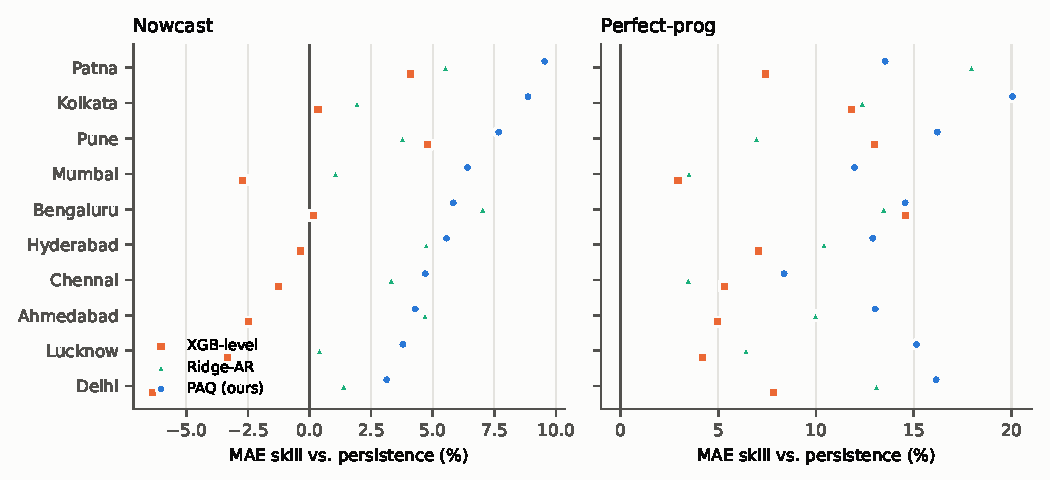
\includegraphics[width=\columnwidth]{fig_city_skill.pdf}
\caption{Per-city MAE skill against persistence. Standard boosting (XGB-level)
falls below zero in six cities in the nowcast setting; PAQ is positive in all ten.}
\label{fig:city}
\end{figure}

\subsection{Standard ML barely beats persistence}
Table~\ref{tab:main} and Fig.~\ref{fig:city} give the headline result. Without
next-day meteorology, standard gradient boosting is \emph{worse} than persistence
overall ($\mathrm{SS}=-1.2\%$) and worst in Delhi ($-6.4\%$), the city where
forecasts matter most. It also has the lowest exceedance F1 of all non-climatology models
(0.819 vs.\ 0.836 for persistence). Linear and random-forest models do slightly better
($+3.0\%$, $+3.4\%$). Climatology is far worse than persistence ($-67\%$), which
confirms that day-to-day memory dominates at this horizon.

PAQ reaches $+6.0\%$ and is positive in every city, from $+3.1\%$ in Delhi to
$+9.5\%$ in Patna. It also has the best category accuracy (0.787). Pooled DM tests favour PAQ
over every baseline except its single-quantile twin (Section~\ref{sec:fact}) ($p<10^{-3}$).
Per city, PAQ is significantly better ($p<0.05$) than persistence in 9/10 cities, than
XGB-level in 9/10 and than Ridge-AR in 4/10. With next-day meteorology all models improve and the
ranking is unchanged. PAQ reaches $+14.9\%$ and beats persistence significantly in 10/10 cities.
Next-day weather therefore roughly doubles to triples the achievable skill, which is consistent with
the strong meteorological control of day-to-day PM$_{2.5}$ variability.

\subsection{Factorial ablation: an interaction}\label{sec:fact}
\begin{table}[t]
\centering
\caption{MAE skill (\%) vs.\ persistence for gradient boosting: target $\times$ loss. Nowcast / perfect-prog.}
\label{tab:factorial}
\begin{tabular}{lcc}
\toprule
Target $\backslash$ Loss & Squared & Median \\
\midrule
Level $z_{t+1}$             & $-1.2$ / 7.8 & 1.5 / 8.3 \\
Change $z_{t+1}-z_t$        & 0.8 / 9.8  & \textbf{6.0} / \textbf{14.6} \\
\bottomrule
\end{tabular}
\end{table}

Table~\ref{tab:factorial} isolates the two design choices. Anchoring on
persistence alone adds about 2 points, and the median loss alone adds 0.5--2.7 points.
Together they add 7.2 (nowcast) and 6.8 (perfect-prog) points over the standard
configuration, more than the sum of the individual effects (4.7 and 2.5 points).
The single-quantile change-median model and PAQ give statistically
indistinguishable point forecasts (DM $p=0.63$). PAQ gets its intervals from the same model
at no extra cost. Practitioners who need only point forecasts can therefore use the simpler
single-quantile model.

\subsection{Mechanism: implicit shrinkage, not better direction}\label{sec:mech}
\begin{table}[t]
\centering
\caption{Nowcast skill (\%) by quartile of the realised change $|z_{t+1}-z_t|$, with the mean absolute predicted change and the share of days on which the predicted direction of change is correct.}
\label{tab:mech}
\setlength{\tabcolsep}{3pt}
\begin{tabular}{lrrrrrr}
\toprule
Model & Q1 & Q2 & Q3 & Q4 & $\overline{|\hat\Delta|}$ & Dir.\ acc \\
\midrule
XGB-level            & $-231.9$ & $-29.7$ & 9.8  & 23.6 & 0.131 & .610 \\
XGB-level (median)   & $-204.5$ & $-23.2$ & 11.8 & 23.0 & 0.119 & .603 \\
XGB-change           & $-197.2$ & $-23.1$ & 11.3 & 21.2 & 0.118 & .606 \\
XGB-change (median)  & $\mathbf{-119.9}$ & $\mathbf{-3.4}$ & \textbf{13.4} & 16.9 & 0.080 & .608 \\
\bottomrule
\end{tabular}
\end{table}

Why do the two ingredients interact? All four boosted variants predict the
\emph{direction} of tomorrow's change equally well (60--61\%, Table~\ref{tab:mech}).
Their difference lies in \emph{magnitude}. The realised change in log concentration is sharply peaked
at zero: 34\% of days have $|\Delta|<0.1$, i.e.\ a change of less than about 10\%, and the excess
kurtosis is 1.9. Its conditional median is therefore pulled towards zero more strongly than its
conditional mean, so the anchored median model makes 32\% smaller moves than the anchored
squared-loss model. This costs a little on days with large changes (Q4: 16.9\% vs.\ 21--24\%) but
removes much of the damage on calm days. On Q1 days every model loses to persistence, but PAQ loses
$-120\%$ compared with $-197$ to $-232\%$. Because calm days are frequent, avoiding these unnecessary moves outweighs
the smaller gains on large-change days, and the net effect is positive. When the target is the level, the median loss
cannot produce this effect, because the reference point it shrinks towards is not persistence.
Anchoring defines \emph{where} to shrink, and the median loss determines \emph{how strongly}.

\subsection{Robustness across seasons, regions and years}
\begin{table}[t]
\centering
\caption{MAE skill (\%) vs.\ persistence by season, region and test year (nowcast / perfect-prog).}
\label{tab:robust}
\setlength{\tabcolsep}{3pt}
\begin{tabular}{lccc}
\toprule
Subset & Ridge-AR & XGB-level & PAQ \\
\midrule
Winter (DJF)        & 6.4 / 17.2 & $-1.2$ / 9.9 & \textbf{7.7} / \textbf{18.6} \\
Pre-monsoon (MAM)   & $-2.0$ / $-1.9$ & $-5.5$ / $-2.7$ & \textbf{2.5} / \textbf{6.0} \\
Monsoon (JJAS)      & 2.2 / 13.0 & 0.9 / 12.8 & \textbf{6.1} / \textbf{17.9} \\
Post-monsoon (ON)   & 3.7 / 11.2 & 1.7 / 10.7 & \textbf{6.8} / \textbf{15.0} \\
\midrule
IGP cities          & 2.3 / 12.6 & $-1.7$ / 7.8 & \textbf{6.1} / \textbf{16.2} \\
Other cities        & 4.0 / 7.9 & $-0.4$ / 7.8 & \textbf{5.8} / \textbf{12.9} \\
\midrule
Test year 2024      & $-0.1$ / 8.8 & $-8.0$ / $-2.4$ & \textbf{3.6} / \textbf{10.3} \\
Test year 2025      & 3.4 / 10.3 & 1.0 / 11.9 & \textbf{6.2} / \textbf{16.2} \\
Test year 2026      & 5.8 / 13.4 & 3.5 / 13.6 & \textbf{8.2} / \textbf{18.1} \\
\bottomrule
\end{tabular}
\end{table}

Table~\ref{tab:robust} breaks skill down by season, region and test year. PAQ is the best model
in every subset and is the only model with positive skill in every row.
\emph{Pre-monsoon} (March--May) is the hardest season for all models. In this season both Ridge-AR
and XGB-level are worse than persistence even with next-day weather, plausibly because
dust and fire events are poorly predictable from local history. Gains are largest in
\emph{winter} and the \emph{monsoon}. In winter, stagnation and ventilation are strongly
controlled by meteorology. In the monsoon, rain-out produces large, weather-driven changes.
With next-day weather the IGP cities gain more than the others (16.2\% vs.\ 12.9\%), which is
consistent with the stronger control of boundary-layer meteorology on polluted, stagnant
winter air. Skill increases with the length of the training record. In 2024, with only
about 17 months of training data, standard boosting is clearly worse than persistence ($-8.0\%$),
while PAQ remains positive ($+3.6\%$). Anchoring is therefore especially valuable when data are scarce,
because the model does not have to learn the persistence relation from limited data.

\subsection{What the model uses}
\begin{table}[t]
\centering
\caption{Share (\%) of total split gain of the PAQ median model by feature group, mean over cities (model trained to end of 2025).}
\label{tab:imp}
\begin{tabular}{lrr}
\toprule
Feature group & Nowcast & Perfect-prog \\
\midrule
Day-$t$ meteorology               & 48.3 & 26.9 \\
Lagged / rolling pollution        & 36.9 & 25.3 \\
Current level \& recent change    &  9.3 &  6.9 \\
Calendar                          &  5.6 &  3.2 \\
Next-day meteorology              &  --  & 37.7 \\
\bottomrule
\end{tabular}
\end{table}

Table~\ref{tab:imp} groups the split-gain importance of the PAQ median model. In the nowcast
setting, meteorology and pollution history contribute almost equally. The most frequent
top-5 features across cities are the lag-1 value $z_{t-1}$ (9 of 10 cities), the day-over-day change in
wind speed (9/10) and the anomaly of today's value from its 30-day mean (8/10). The last of these
captures \emph{mean reversion}: after an unusually high day, the model expects a partial return
towards the recent baseline. With next-day meteorology, the forecast change in wind speed is a top-5
feature in all ten cities and next-day variables take 38\% of the gain. This confirms that the model
mainly learns how tomorrow's \emph{ventilation} differs from today's. Split-gain importance is
a descriptive measure, and these results should not be read as causal attributions.

\subsection{Negative result: an explicit gate is redundant}
\begin{figure}[t]
\centering
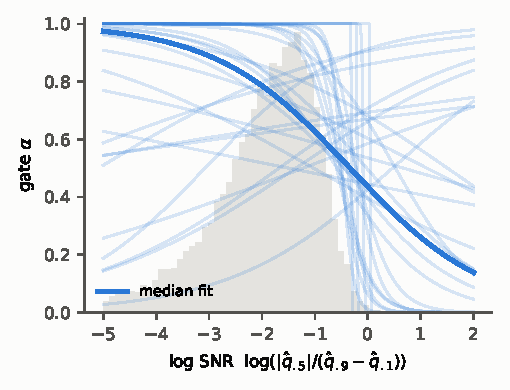
\includegraphics[width=0.8\columnwidth]{fig_gate.pdf}
\caption{Learned SNR gates for each city and fold (thin lines) and their median (thick line), with the distribution of test-set SNR (grey). The gates disagree with each other and mostly have the wrong sign.}
\label{fig:gate}
\end{figure}
If PAQ works by shrinking, an explicit, learned shrinkage should help further.
It does not (Table~\ref{tab:main}). A constant gate and the SNR gate are both
statistically indistinguishable from or slightly worse than PAQ. Moreover, the
fitted SNR-gate slope $b$ has the hypothesised positive sign in only 30\% of
city-folds (nowcast; 27\% perfect-prog), and several fits are degenerate step
functions (Fig.~\ref{fig:gate}). The median loss already performs the shrinkage the gate was
meant to provide. A second-stage gate fitted on a few hundred OOF points mostly fits noise.
We report this negative result because confidence-weighted shrinkage toward a baseline is an
intuitive design that others may otherwise try.

\subsection{Calibrated intervals}
\begin{table}[t]
\centering
\caption{90\% conformal prediction intervals for PAQ (pooled test set). Width in $\mu$g\,m$^{-3}$.}
\label{tab:cov}
\begin{tabular}{llrrr}
\toprule
Setting & Score & Cov. & Worst city & Med.\ width \\
\midrule
Nowcast      & normalised & 0.910 & 0.888 & 28.5 \\
Nowcast      & absolute   & 0.900 & 0.886 & 26.3 \\
Perfect-prog & normalised & 0.912 & 0.878 & 27.0 \\
Perfect-prog & absolute   & 0.895 & 0.874 & 23.2 \\
\bottomrule
\end{tabular}
\end{table}
Both conformal variants achieve close to nominal coverage on the pooled test set,
and no city falls below 87\% (Table~\ref{tab:cov}). This holds although the
exchangeability assumption behind conformal guarantees is only approximately satisfied by
autocorrelated, seasonal data. Both variants are built in log space, so both widen multiplicatively
with concentration. Normalising by the quantile spread $w$ slightly over-covers and gives wider
intervals. We therefore cannot claim an advantage for the adaptive score here. Fig.~\ref{fig:ts}
shows Delhi's 2025--26 winter. The intervals widen during episodes. In this example PAQ also tracks
several winter peaks more closely than level boosting, which tends to smooth them.

\begin{figure*}[t]
\centering
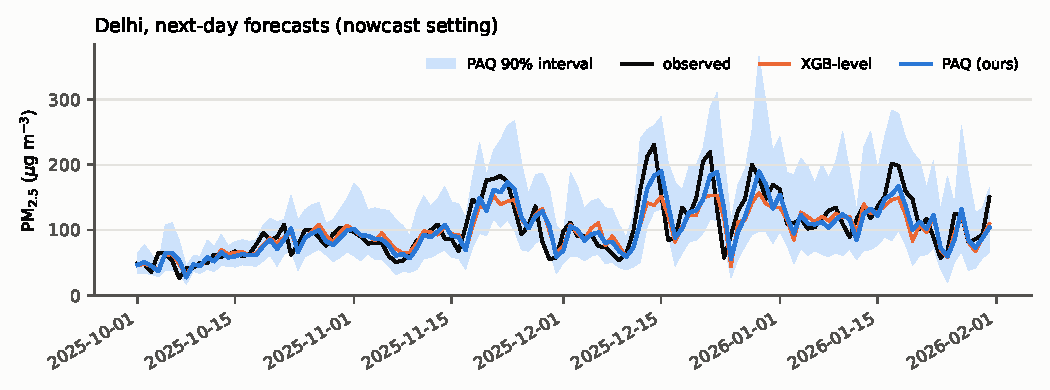
\includegraphics[width=0.85\textwidth]{fig_timeseries.pdf}
\caption{Delhi, Oct 2025--Jan 2026: observed daily PM$_{2.5}$, next-day XGB-level and PAQ forecasts, and PAQ 90\% conformal intervals (nowcast setting).}
\label{fig:ts}
\end{figure*}

%=====================================================================
\section{Discussion}\label{sec:disc}
%=====================================================================
\textbf{Implications for practice.} Three recommendations follow. First, any next-day
air-quality model should report skill against persistence, per city and per season.
A pooled $R^2$ cannot reveal that a model is worse than repeating today's value. Second, the
cheapest improvement to a standard tree pipeline is not a new architecture but a change of
target and loss: predict the change from persistence under a median loss. In XGBoost, LightGBM or
scikit-learn this is a two-line change. Third, PAQ's quantile outputs give, at no extra
cost, prediction intervals that can be conformally calibrated. An advisory system can then
report, for example, the probability of exceeding the national standard instead of a single
number.

\textbf{Why not deeper models?} We deliberately restricted ourselves to tabular
models. The mechanism we identify, a default to persistence plus a robust loss, is not
specific to trees. It is equally available to recurrent or attention models by adding a
residual connection from $z_t$ and training with the pinball loss. Whether deep models
benefit from the same interaction is an open question. Our results suggest that such models
should be compared against an anchored-median tree baseline, not against level-regression
baselines that may themselves be worse than persistence.

\textbf{Relation to CTMs.} Operational systems such as SAFAR and WRF-Chem
\cite{jena2021} simulate the physics, including transport from upwind fires, which local
time-series models cannot see. The approach studied here is complementary. PAQ could
post-process CTM output by using the CTM's forecast change as a feature, and anchoring on
persistence provides a safe fallback when the CTM is biased.

\textbf{Limitations.} (i)~The PM$_{2.5}$ series are CAMS model output, not
station observations. Model fields are spatially smooth and may be more persistent
than point observations, so absolute skill levels may not transfer, and the analysis should
be repeated on CPCB monitoring data. Our code supports the public CPCB city-day format.
(ii)~Perfect-prog uses reanalysis for day $t{+}1$ and therefore overstates the value of
operational weather forecasts. The true value lies between the two settings. (iii)~We use a single
hyperparameter set and a single random seed. The gains are consistent across ten cities, four
seasons and three test years, but we do not report variability over seeds. (iv)~Only a one-day
horizon and one pollutant are studied. At longer horizons persistence weakens and the balance may
shift. (v)~Conformal coverage is only approximately guaranteed for serially dependent data.

%=====================================================================
\section{Conclusion and Future Work}
%=====================================================================
A standard gradient-boosting pipeline for next-day PM$_{2.5}$ in Indian cities
does not reliably beat the persistence forecast. It is worse overall and worse in six of
ten cities. Anchoring the model on persistence and training it under a median loss
beats persistence in all ten cities, all four seasons and all three test years. The
resulting PAQ model is simple, calibrated and interpretable. The two ingredients
interact: their combination implements data-driven shrinkage toward persistence,
which explains why an explicit learned gate brings no further benefit. Future work will
(a)~replicate the study on CPCB station observations, (b)~extend it to 2--3-day
horizons, PM$_{10}$ and the composite AQI, (c)~replace the perfect-prog setting with
archived operational weather forecasts, and (d)~test whether deep sequence models benefit
from the same anchor-and-median design.

\textbf{Reproducibility.} All data are openly available, and the code reproduces every
table and figure: \url{https://github.com/<user>/AQI} % TODO(author)

% Every reference below was checked against Crossref / the publisher record on 2026-10-30.
\begin{thebibliography}{99}
\bibitem{cusworth2018} D.~H.~Cusworth \emph{et al.}, ``Quantifying the influence of agricultural fires in northwest India on urban air pollution in Delhi, India,'' \emph{Environ.\ Res.\ Lett.}, vol.~13, no.~4, p.~044018, 2018, doi:10.1088/1748-9326/aab303.
\bibitem{jena2021} C.~Jena \emph{et al.}, ``Performance of high resolution (400 m) PM$_{2.5}$ forecast over Delhi,'' \emph{Sci.\ Rep.}, vol.~11, p.~4104, 2021, doi:10.1038/s41598-021-83467-8.
\bibitem{inness2019} A.~Inness \emph{et al.}, ``The CAMS reanalysis of atmospheric composition,'' \emph{Atmos.\ Chem.\ Phys.}, vol.~19, no.~6, pp.~3515--3556, 2019, doi:10.5194/acp-19-3515-2019.
\bibitem{masood2020} A.~Masood and K.~Ahmad, ``A model for particulate matter (PM$_{2.5}$) prediction for Delhi based on machine learning approaches,'' \emph{Procedia Comput.\ Sci.}, vol.~167, pp.~2101--2110, 2020, doi:10.1016/j.procs.2020.03.258.
\bibitem{natarajan2024} S.~K.~Natarajan, P.~Shanmurthy, D.~Arockiam, B.~Balusamy, and S.~Selvarajan, ``Optimized machine learning model for air quality index prediction in major cities in India,'' \emph{Sci.\ Rep.}, vol.~14, p.~6795, 2024, doi:10.1038/s41598-024-54807-1.
\bibitem{maltare2023} N.~N.~Maltare and S.~Vahora, ``Air Quality Index prediction using machine learning for Ahmedabad city,'' \emph{Digit.\ Chem.\ Eng.}, vol.~7, p.~100093, 2023, doi:10.1016/j.dche.2023.100093.
\bibitem{pruthi2022} D.~Pruthi and Y.~Liu, ``Low-cost nature-inspired deep learning system for PM$_{2.5}$ forecast over Delhi, India,'' \emph{Environ.\ Int.}, vol.~166, p.~107373, 2022, doi:10.1016/j.envint.2022.107373.
\bibitem{huang2018} C.-J.~Huang and P.-H.~Kuo, ``A deep CNN-LSTM model for particulate matter (PM$_{2.5}$) forecasting in smart cities,'' \emph{Sensors}, vol.~18, no.~7, p.~2220, 2018, doi:10.3390/s18072220.
\bibitem{zhou2024} S.~Zhou, W.~Wang, L.~Zhu, Q.~Qiao, and Y.~Kang, ``Deep-learning architecture for PM$_{2.5}$ concentration prediction: A review,'' \emph{Environ.\ Sci.\ Ecotechnol.}, vol.~21, p.~100400, 2024, doi:10.1016/j.ese.2024.100400.
\bibitem{chianese2026} E.~Chianese and A.~Riccio, ``Air-quality forecasting across monitoring, predictor, and validation regimes: A systematic mapping review and decision framework,'' \emph{Forecasting}, vol.~8, no.~4, p.~72, 2026, doi:10.3390/forecast8040072.
\bibitem{murphy1988} A.~H.~Murphy, ``Skill scores based on the mean square error and their relationships to the correlation coefficient,'' \emph{Mon.\ Weather Rev.}, vol.~116, no.~12, pp.~2417--2424, 1988.
\bibitem{rasp2020} S.~Rasp \emph{et al.}, ``WeatherBench: A benchmark data set for data-driven weather forecasting,'' \emph{J.\ Adv.\ Model.\ Earth Syst.}, vol.~12, no.~11, e2020MS002203, 2020, doi:10.1029/2020MS002203.
\bibitem{hyndman2006} R.~J.~Hyndman and A.~B.~Koehler, ``Another look at measures of forecast accuracy,'' \emph{Int.\ J.\ Forecast.}, vol.~22, no.~4, pp.~679--688, 2006, doi:10.1016/j.ijforecast.2006.03.001.
\bibitem{agarwal2023} A.~Agarwal and M.~Sahu, ``Forecasting PM$_{2.5}$ concentrations using statistical modeling for Bengaluru and Delhi regions,'' \emph{Environ.\ Monit.\ Assess.}, vol.~195, no.~4, p.~502, 2023, doi:10.1007/s10661-023-11045-8.
\bibitem{wang2020gnn} S.~Wang, Y.~Li, J.~Zhang, Q.~Meng, L.~Meng, and F.~Gao, ``PM2.5-GNN: A domain knowledge enhanced graph neural network for PM2.5 forecasting,'' in \emph{Proc.\ 28th Int.\ Conf.\ Advances in Geographic Information Systems (SIGSPATIAL)}, 2020, pp.~163--166, doi:10.1145/3397536.3422208.
\bibitem{rybarczyk2018} Y.~Rybarczyk and R.~Zalakeviciute, ``Machine learning approaches for outdoor air quality modelling: A systematic review,'' \emph{Appl.\ Sci.}, vol.~8, no.~12, p.~2570, 2018, doi:10.3390/app8122570.
\bibitem{bai2018} L.~Bai, J.~Wang, X.~Ma, and H.~Lu, ``Air pollution forecasts: An overview,'' \emph{Int.\ J.\ Environ.\ Res.\ Public Health}, vol.~15, no.~4, p.~780, 2018, doi:10.3390/ijerph15040780.
\bibitem{makridakis2018} S.~Makridakis, E.~Spiliotis, and V.~Assimakopoulos, ``Statistical and machine learning forecasting methods: Concerns and ways forward,'' \emph{PLOS ONE}, vol.~13, no.~3, e0194889, 2018, doi:10.1371/journal.pone.0194889.
\bibitem{diebold1995} F.~X.~Diebold and R.~S.~Mariano, ``Comparing predictive accuracy,'' \emph{J.\ Bus.\ Econ.\ Statist.}, vol.~13, no.~3, pp.~253--263, 1995, doi:10.1080/07350015.1995.10524599.
\bibitem{harvey1997} D.~Harvey, S.~Leybourne, and P.~Newbold, ``Testing the equality of prediction mean squared errors,'' \emph{Int.\ J.\ Forecast.}, vol.~13, no.~2, pp.~281--291, 1997, doi:10.1016/S0169-2070(96)00719-4.
\bibitem{koenker1978} R.~Koenker and G.~Bassett, ``Regression quantiles,'' \emph{Econometrica}, vol.~46, no.~1, pp.~33--50, 1978, doi:10.2307/1913643.
\bibitem{chen2016} T.~Chen and C.~Guestrin, ``XGBoost: A scalable tree boosting system,'' in \emph{Proc.\ 22nd ACM SIGKDD}, 2016, pp.~785--794, doi:10.1145/2939672.2939785.
\bibitem{murad2021} A.~Murad, F.~A.~Kraemer, K.~Bach, and G.~Taylor, ``Probabilistic deep learning to quantify uncertainty in air quality forecasting,'' \emph{Sensors}, vol.~21, no.~23, p.~8009, 2021, doi:10.3390/s21238009.
\bibitem{lei2018} J.~Lei, M.~G'Sell, A.~Rinaldo, R.~J.~Tibshirani, and L.~Wasserman, ``Distribution-free predictive inference for regression,'' \emph{J.\ Amer.\ Statist.\ Assoc.}, vol.~113, no.~523, pp.~1094--1111, 2018, doi:10.1080/01621459.2017.1307116.
\bibitem{romano2019} Y.~Romano, E.~Patterson, and E.~J.~Cand\`es, ``Conformalized quantile regression,'' in \emph{Adv.\ Neural Inf.\ Process.\ Syst.\ (NeurIPS)}, vol.~32, 2019.
\bibitem{breiman2001} L.~Breiman, ``Random forests,'' \emph{Mach.\ Learn.}, vol.~45, no.~1, pp.~5--32, 2001, doi:10.1023/A:1010933404324.
\bibitem{hersbach2020} H.~Hersbach \emph{et al.}, ``The ERA5 global reanalysis,'' \emph{Q.\ J.\ R.\ Meteorol.\ Soc.}, vol.~146, no.~730, pp.~1999--2049, 2020, doi:10.1002/qj.3803.
\bibitem{openmeteo} P.~Zippenfenig, ``Open-Meteo.com Weather API,'' Zenodo, 2024, doi:10.5281/zenodo.7970649.
\end{thebibliography}

\end{document}
